\documentclass[output=paper]{langsci/langscibook}
\title{Language intertwined across multiple timescales: {Processing}, acquisition and evolution}
\ChapterDOI{10.5281/zenodo.573775}
\author{Morten H. Christiansen\affiliation{Department of Psychology, Cornell University, Ithaca, NY, USA\newline Centre for Interacting Minds, Aarhus University, Denmark}}
\rohead{Language intertwined across multiple timescales}
\maketitle
\begin{document} 
\is{timescales} \is{processing} \is{acquisition} \is{language evolution}
Theories of language invoke different types of causal dependencies to explain a variety of linguistic phenomena, ranging from typological patterns (e.g., ``verb-final languages tend to have postpositions," \citealt{Greenberg1966OrderMeaningfulElements}) to psycholinguistic regularities (e.g., ``hearing a passive construction increases the likelihood of producing one," \citealt{Bock1986}). Several chapters in this volume provide important insights into such dependencies across a variety of domains (see, for example, chapters by Cristofaro, Culbertson, Dediu, Hyman, and Rice). This chapter, however, concerns itself with a different kind of dependency: the fundamental theoretical interdependencies between different timescales of language, from processing to acquisition to evolution. 

\is{generative linguistics}
In the mainstream generative grammar tradition, possible interdependencies between language processing, acquisition and evolution are rarely ever explored \citep[but see][]{Pinker1994,Jackendoff2002}. This is likely a consequence of Chomsky’s methodological dictums that the study of language proper should be separated from how it is used and processed \citep{Chomsky1965}, acquired over development \citep{Chomsky1975}, and how it evolved \citep{Chomsky2005}. \citet{Christiansen2016}  refer to the theoretical impact of these methodological dictums as “Chomsky’s hidden legacy”, and note that its influence has gone well beyond generative approaches. For example, typological and usage-based approaches to language processing typically downplay issues related to the acquisition and evolution of language \citep[e.g.,][]{Clark1996,Hawkins1994}. Similarly, work on language acquisition tends not to consider questions pertaining to the processing and evolution of language \citep[e.g.,][]{Cowie1999,Hirsh-Pasek1996,OGrady1997}, and studies of language evolution usually pay little attention to research on language acquisition and processing \citep[e.g.,][]{Botha2003,Burling2005,Corballis2002,Dunbar1998,Lieberman2000}. In contrast, \citet{Christiansen2016} argue that there are strong theoretical constraints between the processing, acquisition and evolution of language--allowing each to shed light on the others--and that key questions within each area can only be fully addressed through an integrated approach. As an example, I briefly discuss how the immediacy of language processing has implications for both language acquisition and evolution. \is{processing} \is{acquisition} \is{language evolution}

\section{The Now-or-Never bottleneck}
\is{acoustics} \is{now-or-never bottleneck} \is{chunk-and-pass processing}
Language happens in the here-and-now. Our memory for acoustic information is incredibly short-lived, disappearing within less than 100 msec \citep{Remez2010}. At the same time spoken language comes at us at a very rapid rate, at about 10-15 phonemes per second \citep{Studdert-Kennedy1986}, with the further complication that our auditory system is only able to keep track of about 10 separate (non-speech) sounds per second \citep{Miller1948}. To make matters worse, our ability to keep track of sound sequences is also very limited: we are able to recall less than four non-speech sounds \citep{Warren1969} and only four to seven unrelated linguistic items \citep{Cowan2000,Miller1956}. Thus, during a normal conversation, we are faced with an immense challenge by the combined effects of poor acoustic memory, fast input, and severely limited sequence memory.\footnote{ Communication using sign language involves a similar problem (see \citealt{ChristiansenInPress} for discussion)} As a consequence of this \textsc{Now-or-Never bottleneck } \citep{ChristiansenInPress}, new material will constantly overwrite and interfere with previous material unless it is processed immediately.
 
\largerpage[-2] 
The Now-or-Never bottleneck has direct implications for language processing. To deal with the immediacy of language, \citet{ChristiansenInPress} suggest that the language system must engage in \textsc{Chunk-and-Pass} processing: compress and recode language input as rapidly as possible into increasingly more abstract levels of linguistic representation, from sound-based units to words (or word combinations) to discourse-level representations. This passing up of chunks allows for increasingly longer retention of linguistic information at higher levels of linguistic abstraction, consistent with recent neuroimaging data \citep[e.g.,][]{Ding2016,Stephens2013}.

\newpage 
\is{chunk-and-pass processing} \is{biases} \is{local dependencies} \is{garden-path effects} The time-sensitive nature of Chunk-and-Pass processing leads to a strong pressure toward incremental processing because chunking will primarily happen across neighboring units, resulting in a bias toward local dependencies \citep[in line with evidence for garden path effects in language comprehension; e.g.,][]{Bever1970}. The multiple levels of linguistic structure that result from the Chunk-and-Pass process provides a possible processing-based explanation for why linguistic theories tend to be couched in terms of multiple levels of representation, from phonology and morphology to syntax and discourse.\footnote{ Although this perspective is consistent with standard levels of linguistic abstraction, from phonology through syntax to pragmatics, a complete model might incorporate more fine-grained levels that, for example, would distinguish between multiple levels of discourse representation \citep[e.g., as in][]{Enfield2013}.} Importantly, though, in the proposed framework, higher levels of representations will contain less of the original detail of the input as it becomes more compressed through repeated Chunk-and-Pass processing.
 
\largerpage[-1] 
Because the Now-or-Never bottleneck prevents any significant backtracking, the language system employs prediction\is{prediction}\is{processing} to use as much available information as possible to be right the first time. In doing so, the processing system will build the most abstract and complete representation that is justified, given the linguistic input--a “good-enough” representation \citep{Ferreira2002,Ferreira2007}. Through prediction, top-down information from discourse expectations, world knowledge, and so on, is used to guide the incremental interpretation of linguistic input. Language production follows the same principles but in the opposite direction, from discourse representations of the intended message and intonational phrases to words and articulatory motor commands (see \citealt{ChaterSqueezeInPress,ChaterLanguageInPress} for discussion). \is{production}

\is{acquisition} \is{processing} \is{mini-linguist} \is{now-or-never bottleneck} The effects of the Now-and-Never bottleneck go beyond the timescale of processing to the timescale of acquisition. In order to become a competent language user, the child must learn how to create and integrate the right chunks as rapidly as possible, before the input is gone. From this perspective, language acquisition does \textit{not} consist in identifying the right grammar but rather, \textit{language acquisition is learning to process}, to become more efficient at Chunk-and-Pass processing. That is, the child is not a “mini-linguist” but a developing language user, acquiring the necessary skills to comprehend and produce language. To deal with the Now-or-Never bottleneck, the child must learn in the “here-and-now,” relying only on currently available information, instead of abstracting over large swaths of data\footnote{ The Now-or-Never bottleneck thus has important implications for computational models of language, many of which use so-called batch-learning either over large corpora \citep[e.g.,][]{Perfors2010} or large memory windows \citep[e.g.,][]{Kolodny2015} incompatible with psychological constraints on memory. In contrast, the Chunk-Based Learner \citep{McCauley2014,McCauley2016} was developed with the Now-and-Never bottleneck in mind, providing a computational account of aspects of early language acquisition, including the interconnected nature of comprehension and production \citep{ChaterLanguageInPress}.}. Learning is therefore local and piecemeal, constrained by limited memory, in line with item-based approaches to language acquisition \citep[e.g.,][]{Tomasello2003constructing}. Children gradually learn to apply top-down knowledge to facilitate Chunk-and-Pass processing via prediction. Thus, predictive abilities emerge over time as children develop their chunking skills and learn to rapidly apply the multiple constraints that are crucial to adult incremental processing \citep{Borovsky2012}. \is{acquisition} \is{prediction}

The theoretical impact of the Now-or-Never bottleneck\is{now-or-never bottleneck}\is{timescales}\is{language evolution}\is{language change} not only affects the timescales of processing and acquisition, but also extends to the longer timescales of language evolution and change. Given the hypothesis that language evolution may be explained primarily by the cultural evolution of linguistic structure rather than biological adaptations for language \is{cultural evolution} (e.g., \citealt{Christiansen2008,Hurford1999,Smith2008}; for a review, see \citealt{DediuEtAl2013}), we might expect that linguistic patterns that can be processed through the bottleneck will tend to proliferate. That is, language is a product of piecemeal tinkering, with the long-term evolution of language resulting from the compounding of a myriad local short-term processes of language change. This means that \textit{language change is item-based} in nature, with specific changes arising from constraints on Chunk-and-Pass processing--both within and across individuals--providing a possible cognitive foundation for grammaticalization. \is{grammaticalization} 

 \is{now-or-never bottleneck} \is{reduction} \is{erosion} \is{syntacticization} \is{semantic bleaching} The Now-or-Never bottleneck provides a constant pressure towards reduction and erosion across different levels of linguistic representation, from discourse syntacticization and semantic bleaching to morphological reduction and phonetic erosion (see \citealt{ChristiansenInPress} for further discussion). Language change, more broadly, will be local at the level of individual chunks, consistent with theories of lexical diffusion suggesting that sound change originates in a small set of words and then spreads throughout the vocabulary \citep[e.g.,][]{Wang1977}. Similarly, morpho-syntactic change is also predicted to be local in nature, resulting in what \citet{ChristiansenInPress} term “constructional diffusion.”  \is{lexical diffusion} \is{constructional diffusion}

\is{language evolution} \is{language change} Importantly, the process of piecemeal tinkering that drives item-based language change is subject to constraints deriving not only from Chunk-and-Pass processing but also from the specific trajectory of cultural evolution that a language follows. More generally, in this perspective, there is no sharp distinction between language evolution and language change: language evolution is simply the result of language change writ large \citep[see also][]{Heine2007}, constrained by processing and acquisition (see \citealt{Christiansen2016} for more details).

\largerpage
\section{Language intertwined across multiple timescales}
\begin{figure}[b]  
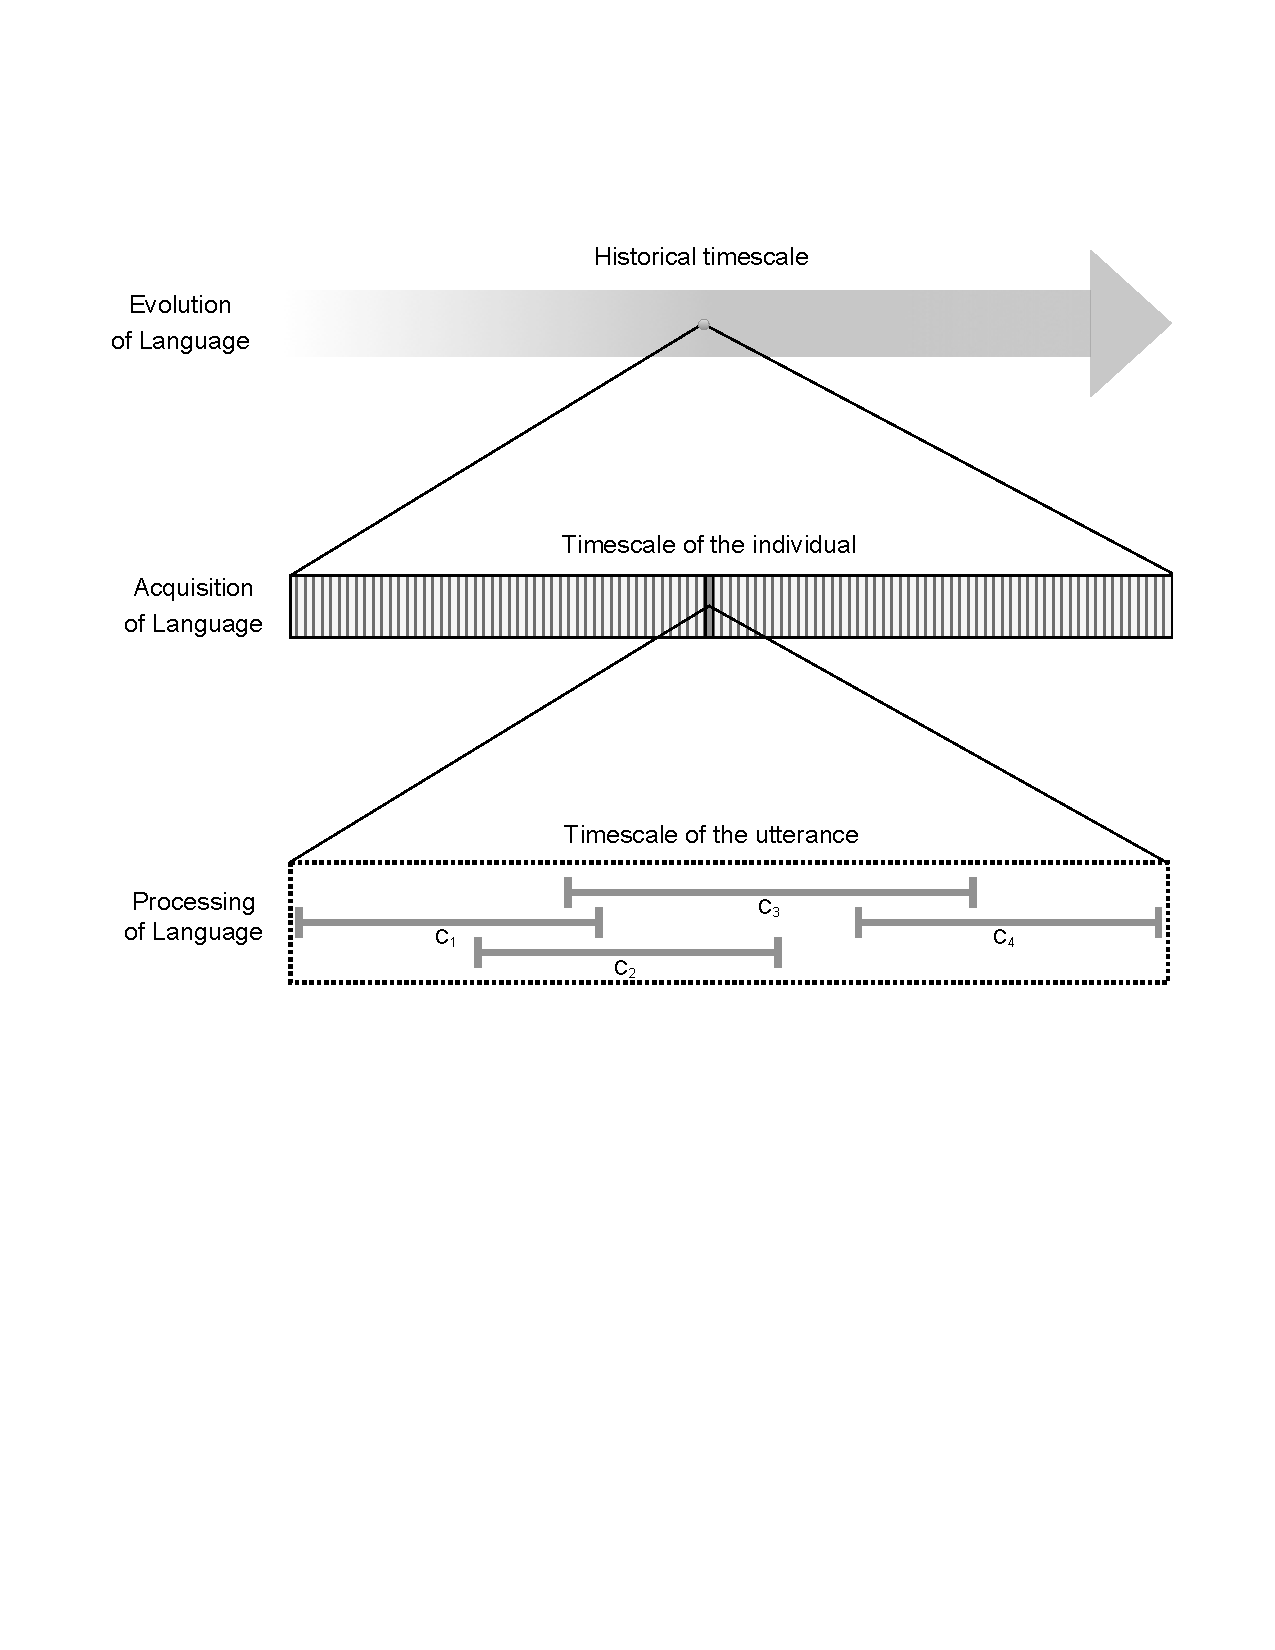
\includegraphics[height=0.45\textheight]{figures/cropped_christiansen_timescales.pdf}
\caption{Illustration of how Chunk-and-Pass processing at the utterance level (with the C\textsubscript{1-4} referring to different chunks) constrains the acquisition of language by the individual, which, in turn, influences how language evolves through learning and use by groups of individuals on a historical timescale. Adapted from \citet{Christiansen2016}.
}
\label{fig:christensen:1}
\end{figure}
\is{now-or-never bottleneck} \is{processing} In this chapter, I have discussed how the Now-or-Never bottleneck not only provides constraints on the processing of language but also on the nature of language acquisition and evolution (with further implications for the structure of language itself, as discussed in \citealt{Christiansen2016,ChristiansenInPress}). \figref{fig:christensen:1} provides an illustration of how the Now-or-Never bottleneck affects language across these different timescales.



At the timescale of the utterance (seconds), Chunk-and-Pass processing carves the input--or output--into chunks at various levels of linguistic abstraction. At the timescale of the individual (tens of years), these chunks provide the comprehension and production events from which children learn (and adults update) their ability to process language. And, on a historical timescale (hundreds or thousands of years), each learner is part of a community of language users that together change language, based on patterns that are easy to acquire and process. Of course, the Now-or-Never bottleneck works together with other constraints deriving from the brain and body to shape the cultural evolution of language \citep{Christiansen2008,Christiansen2016}, where the brain and body are embedded in a social network of interactions. Thus, to reach a complete understanding of how language works, we need to study it as intertwined across the multiple timescales of processing, acquisition and evolution.
 

\section*{Acknowledgments}


Thanks to Erin Isbilen for comments on a previous version of this chapter.

{\sloppy
\printbibliography[heading=subbibliography,notkeyword=this]
}

\end{document}
